% Options for packages loaded elsewhere
\PassOptionsToPackage{unicode}{hyperref}
\PassOptionsToPackage{hyphens}{url}
%
\documentclass[
]{report}
\usepackage{lmodern}
\usepackage{amssymb,amsmath}
\usepackage{ifxetex,ifluatex}
\ifnum 0\ifxetex 1\fi\ifluatex 1\fi=0 % if pdftex
  \usepackage[T1]{fontenc}
  \usepackage[utf8]{inputenc}
  \usepackage{textcomp} % provide euro and other symbols
\else % if luatex or xetex
  \usepackage{unicode-math}
  \defaultfontfeatures{Scale=MatchLowercase}
  \defaultfontfeatures[\rmfamily]{Ligatures=TeX,Scale=1}
\fi
% Use upquote if available, for straight quotes in verbatim environments
\IfFileExists{upquote.sty}{\usepackage{upquote}}{}
\IfFileExists{microtype.sty}{% use microtype if available
  \usepackage[]{microtype}
  \UseMicrotypeSet[protrusion]{basicmath} % disable protrusion for tt fonts
}{}
\makeatletter
\@ifundefined{KOMAClassName}{% if non-KOMA class
  \IfFileExists{parskip.sty}{%
    \usepackage{parskip}
  }{% else
    \setlength{\parindent}{0pt}
    \setlength{\parskip}{6pt plus 2pt minus 1pt}}
}{% if KOMA class
  \KOMAoptions{parskip=half}}
\makeatother
\usepackage{xcolor}
\IfFileExists{xurl.sty}{\usepackage{xurl}}{} % add URL line breaks if available
\IfFileExists{bookmark.sty}{\usepackage{bookmark}}{\usepackage{hyperref}}
\hypersetup{
  pdfauthor={Melinda Yager, Jade Schmidt, Dr.~Stacey Hancock},
  hidelinks,
  pdfcreator={LaTeX via pandoc}}
\urlstyle{same} % disable monospaced font for URLs
\usepackage{color}
\usepackage{fancyvrb}
\newcommand{\VerbBar}{|}
\newcommand{\VERB}{\Verb[commandchars=\\\{\}]}
\DefineVerbatimEnvironment{Highlighting}{Verbatim}{commandchars=\\\{\}}
% Add ',fontsize=\small' for more characters per line
\usepackage{framed}
\definecolor{shadecolor}{RGB}{248,248,248}
\newenvironment{Shaded}{\begin{snugshade}}{\end{snugshade}}
\newcommand{\AlertTok}[1]{\textcolor[rgb]{0.94,0.16,0.16}{#1}}
\newcommand{\AnnotationTok}[1]{\textcolor[rgb]{0.56,0.35,0.01}{\textbf{\textit{#1}}}}
\newcommand{\AttributeTok}[1]{\textcolor[rgb]{0.77,0.63,0.00}{#1}}
\newcommand{\BaseNTok}[1]{\textcolor[rgb]{0.00,0.00,0.81}{#1}}
\newcommand{\BuiltInTok}[1]{#1}
\newcommand{\CharTok}[1]{\textcolor[rgb]{0.31,0.60,0.02}{#1}}
\newcommand{\CommentTok}[1]{\textcolor[rgb]{0.56,0.35,0.01}{\textit{#1}}}
\newcommand{\CommentVarTok}[1]{\textcolor[rgb]{0.56,0.35,0.01}{\textbf{\textit{#1}}}}
\newcommand{\ConstantTok}[1]{\textcolor[rgb]{0.00,0.00,0.00}{#1}}
\newcommand{\ControlFlowTok}[1]{\textcolor[rgb]{0.13,0.29,0.53}{\textbf{#1}}}
\newcommand{\DataTypeTok}[1]{\textcolor[rgb]{0.13,0.29,0.53}{#1}}
\newcommand{\DecValTok}[1]{\textcolor[rgb]{0.00,0.00,0.81}{#1}}
\newcommand{\DocumentationTok}[1]{\textcolor[rgb]{0.56,0.35,0.01}{\textbf{\textit{#1}}}}
\newcommand{\ErrorTok}[1]{\textcolor[rgb]{0.64,0.00,0.00}{\textbf{#1}}}
\newcommand{\ExtensionTok}[1]{#1}
\newcommand{\FloatTok}[1]{\textcolor[rgb]{0.00,0.00,0.81}{#1}}
\newcommand{\FunctionTok}[1]{\textcolor[rgb]{0.00,0.00,0.00}{#1}}
\newcommand{\ImportTok}[1]{#1}
\newcommand{\InformationTok}[1]{\textcolor[rgb]{0.56,0.35,0.01}{\textbf{\textit{#1}}}}
\newcommand{\KeywordTok}[1]{\textcolor[rgb]{0.13,0.29,0.53}{\textbf{#1}}}
\newcommand{\NormalTok}[1]{#1}
\newcommand{\OperatorTok}[1]{\textcolor[rgb]{0.81,0.36,0.00}{\textbf{#1}}}
\newcommand{\OtherTok}[1]{\textcolor[rgb]{0.56,0.35,0.01}{#1}}
\newcommand{\PreprocessorTok}[1]{\textcolor[rgb]{0.56,0.35,0.01}{\textit{#1}}}
\newcommand{\RegionMarkerTok}[1]{#1}
\newcommand{\SpecialCharTok}[1]{\textcolor[rgb]{0.00,0.00,0.00}{#1}}
\newcommand{\SpecialStringTok}[1]{\textcolor[rgb]{0.31,0.60,0.02}{#1}}
\newcommand{\StringTok}[1]{\textcolor[rgb]{0.31,0.60,0.02}{#1}}
\newcommand{\VariableTok}[1]{\textcolor[rgb]{0.00,0.00,0.00}{#1}}
\newcommand{\VerbatimStringTok}[1]{\textcolor[rgb]{0.31,0.60,0.02}{#1}}
\newcommand{\WarningTok}[1]{\textcolor[rgb]{0.56,0.35,0.01}{\textbf{\textit{#1}}}}
\usepackage{longtable,booktabs}
% Correct order of tables after \paragraph or \subparagraph
\usepackage{etoolbox}
\makeatletter
\patchcmd\longtable{\par}{\if@noskipsec\mbox{}\fi\par}{}{}
\makeatother
% Allow footnotes in longtable head/foot
\IfFileExists{footnotehyper.sty}{\usepackage{footnotehyper}}{\usepackage{footnote}}
\makesavenoteenv{longtable}
\usepackage{graphicx}
\makeatletter
\def\maxwidth{\ifdim\Gin@nat@width>\linewidth\linewidth\else\Gin@nat@width\fi}
\def\maxheight{\ifdim\Gin@nat@height>\textheight\textheight\else\Gin@nat@height\fi}
\makeatother
% Scale images if necessary, so that they will not overflow the page
% margins by default, and it is still possible to overwrite the defaults
% using explicit options in \includegraphics[width, height, ...]{}
\setkeys{Gin}{width=\maxwidth,height=\maxheight,keepaspectratio}
% Set default figure placement to htbp
\makeatletter
\def\fps@figure{htbp}
\makeatother
\setlength{\emergencystretch}{3em} % prevent overfull lines
\providecommand{\tightlist}{%
  \setlength{\itemsep}{0pt}\setlength{\parskip}{0pt}}
\setcounter{secnumdepth}{5}
\usepackage{booktabs}
\usepackage{geometry}
\usepackage[none]{hyphenat}
\usepackage{titlesec}
\usepackage{longtable}
\usepackage{longtable}
\usepackage{xcolor}
\usepackage{setspace}

\pagestyle{plain}

%%%% Set margins
\setlength{\topmargin}{-1cm}
\addtolength{\evensidemargin}{-1cm}
\addtolength{\oddsidemargin}{-1cm}
\addtolength{\textheight}{3cm}
\addtolength{\textwidth}{2cm}

% Spacing for reading guides
\newcommand{\rgs}{\vspace{12pt}} % Vertical space
\newcommand{\rgi}{\hspace{24pt}}  % Indent

\newcommand\latexcode[1]{#1}

\renewcommand*{\chaptername}{Activity}

\titleformat{\chapter}[display]
{\bfseries\Large}
{\filleft\MakeUppercase{\chaptertitlename} \Huge\thechapter}
{3ex}
{\titlerule
\vspace{1.5ex}%
\filright}
[\vspace{1.5ex}%
\titlerule]
\titlespacing*{\chapter}{0pt}{-40pt}{20pt}
\ifluatex
  \usepackage{selnolig}  % disable illegal ligatures
\fi
\usepackage[]{natbib}
\bibliographystyle{plainnat}

\title{\textbf{STAT 216 Coursepack}\\
~\\
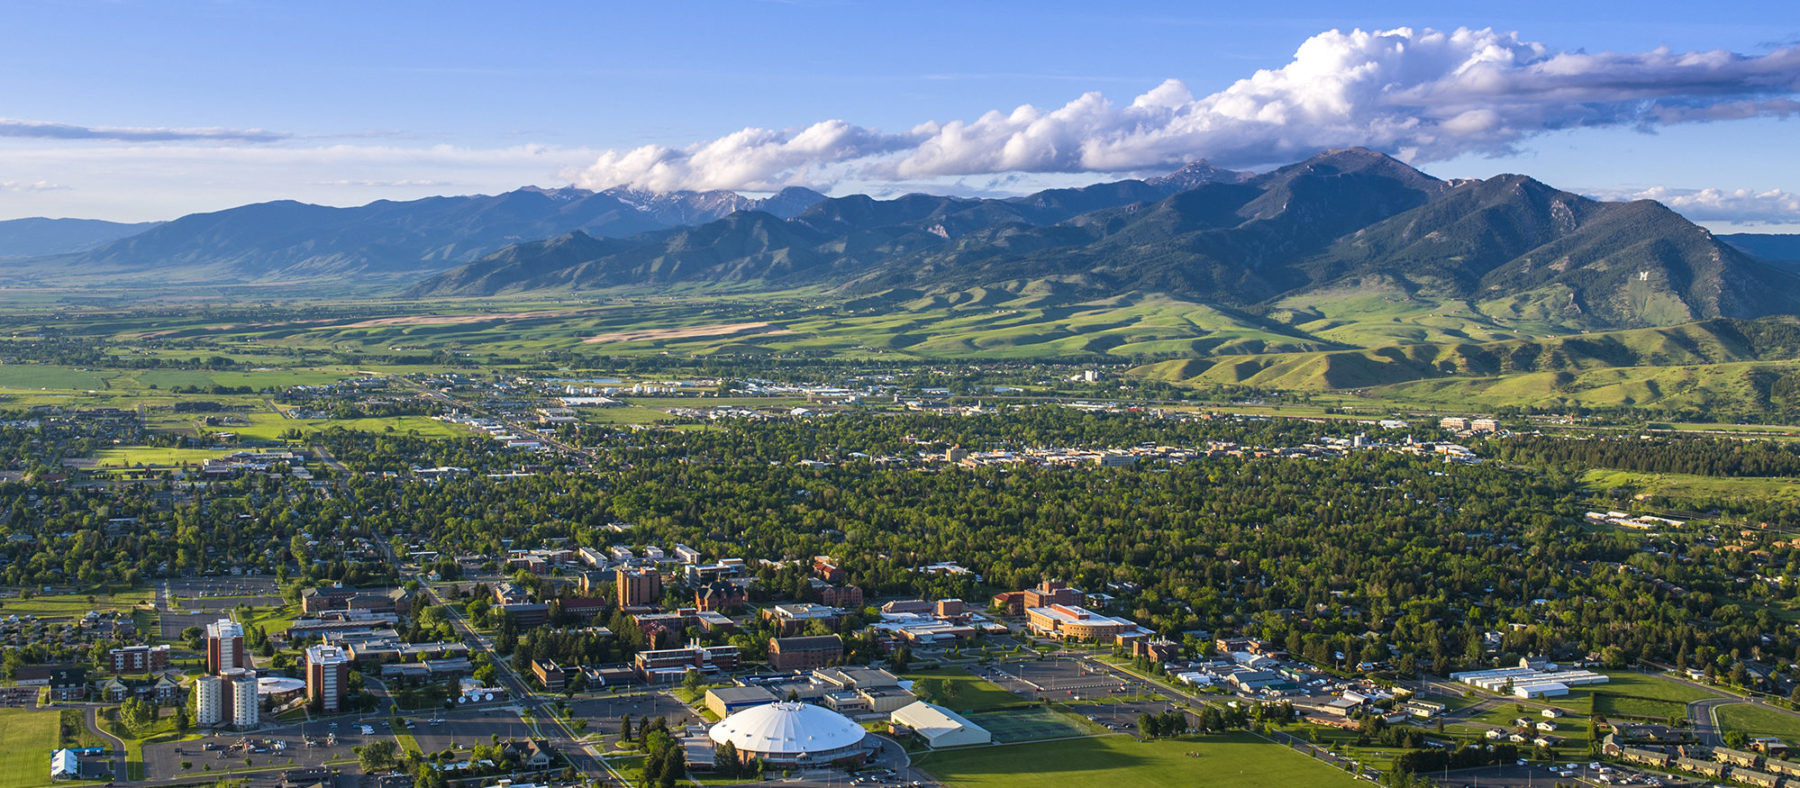
\includegraphics[width=5in,height=\textheight]{images/msu-campus.jpg}}
\usepackage{etoolbox}
\makeatletter
\providecommand{\subtitle}[1]{% add subtitle to \maketitle
  \apptocmd{\@title}{\par {\large #1 \par}}{}{}
}
\makeatother
\subtitle{Spring 2021\\
Montana State University}
\author{Melinda Yager, Jade Schmidt, Dr.~Stacey Hancock}
\date{}

\begin{document}
\maketitle

\newpage
\thispagestyle{empty}

This resource was developed by Melinda Yager, Jade Schmidt, and Stacey Hancock in 2021 to accompany the online textbook: Carnegie, N., Hancock, S., Meyer, E., Schmidt, J., and Yager, M. (2021). \emph{Montana State Introductory Statistics with R}. Montana State University. \url{https://mtstateintrostats.github.io/IntroStatTextbook/}.

This resource is released under a \href{https://creativecommons.org/licenses/by-nc-sa/4.0/}{Creative Commons BY-NC-SA 4.0} license unless otherwise noted.

\setcounter{tocdepth}{1}
\tableofcontents
\setcounter{page}{1}

\newpage

\hypertarget{preface}{%
\chapter*{Preface}\label{preface}}
\addcontentsline{toc}{chapter}{Preface}

This coursepack accompanies the textbook for STAT 216: Introduction to Statistics at Montana State University, which can be found at \url{https://mtstateintrostats.github.io/IntroStatTextbook/}. The syllabus for the course (including the course calendar), data sets, and links to D2L Brightspace, Gradescope, and the MSU RStudio server can be found on the course webpage: \url{https://math.montana.edu/courses/s216/}.
Videos assigned in the course calendar and other notes and review materials are linked in D2L.

Each of the activities in this workbook is designed to target specific learning outcomes of the course, giving you practice with important statistical concepts in a group setting with instructor guidance. In addition to the in-class activities for the course, the coursepack includes reading guides to aid in taking notes while you complete the required readings and videos. Bring this workbook with you to class each week, and take notes in the workbook as you would your own notes. A well-written complete workbook will provide an optimal study guide for exams!

The activities in this coursepack are broken into three sections: pre-class, in-class, and after class. Read through the introduction for each activity and complete the pre-class questions before attending class each week. In class, you will work through the in-class section with your group and instructor. After class, you will complete the out-of-class part of the activity.

STAT 216 is a 3-credit blended course. Rather than meeting for a total of 150 structured minutes in class per week, students meet with their instructor and cohort of classmates for 50 minutes of class per week. The other 100 minutes typically spent in class are instead spent outside of class watching instructor video lectures, reading the textbook, working through case studies, and participating in online discussion with your classmates. This structure serves two purposes: (1) enhance the safety of our community during the COVID-19 pandemic, and (2) provide additional flexibility for students to create their own schedule and make their own decisions on how they learn best.

In our experience, it takes six to nine hours per week outside of class to achieve a good grade in STAT 216 -- this means six to nine hours outside of the 150 minutes of time set aside for learning course material each week. By ``good'' we mean at least a C because a grade of C- or below does not count toward fulfilling degree requirements. Many of you set your goals higher than just getting a C, and we fully support that. You
need roughly nine hours per week to review past activities, read feedback on previous assignments, complete current assignments, and prepare for the next day's class. A typical week in the life of a STAT 216 student looks like:

\begin{itemize}
\tightlist
\item
  \emph{Prior to class meeting}:

  \begin{itemize}
  \tightlist
  \item
    Read assigned sections of the textbook, using the provided reading guides to take notes on the material.
  \item
    Watch assigned videos on that week's content, pausing to take notes and answer video quiz questions.
  \item
    Read through the introduction to the week's in-class activity and complete the pre-class questions.
  \item
    Read through the week's homework assignment and note any questions you may have on the content.
  \end{itemize}
\item
  \emph{During class meeting}:

  \begin{itemize}
  \tightlist
  \item
    Work through in-class activity with your classmates and instructor, taking detailed notes on your answers to each question in the activity.
  \end{itemize}
\item
  \emph{After class meeting}:

  \begin{itemize}
  \tightlist
  \item
    Complete the out-of-class part of the activity, plus any additional parts of the activity you did not complete in class.
  \item
    Review the posted activity solutions and wrap-up videos, and take notes on key points.
  \item
    Finish watching any remaining assigned videos or readings for the week.
  \item
    Read through the week's case study and post case study discussion posts on D2L.
  \item
    Complete the week's homework assignment.
  \end{itemize}
\end{itemize}

\hypertarget{inference-for-two-categorical-variables-hypothesis-testing}{%
\chapter{Inference for Two Categorical Variables: Hypothesis Testing}\label{inference-for-two-categorical-variables-hypothesis-testing}}

\hypertarget{reading-guide-hypothesis-testing-for-a-difference-in-proportions}{%
\section{Reading Guide: Hypothesis Testing for a Difference in Proportions}\label{reading-guide-hypothesis-testing-for-a-difference-in-proportions}}

\hypertarget{sections-5.4.1-and-5.4.2-simulation-tests-for-a-difference-in-proportions-two-sided-hypotheses}{%
\subsection*{Sections 5.4.1 and 5.4.2 (Simulation tests for a difference in proportions; Two-sided hypotheses)}\label{sections-5.4.1-and-5.4.2-simulation-tests-for-a-difference-in-proportions-two-sided-hypotheses}}
\addcontentsline{toc}{subsection}{Sections 5.4.1 and 5.4.2 (Simulation tests for a difference in proportions; Two-sided hypotheses)}

\textbf{Videos}

\begin{itemize}
\tightlist
\item
  5.4
\item
  TwoPropSim
\end{itemize}

\setstretch{1.25}

\hypertarget{reminders-from-previous-sections}{%
\subsubsection*{Reminders from previous sections}\label{reminders-from-previous-sections}}
\addcontentsline{toc}{subsubsection}{Reminders from previous sections}

\(n\) = sample size

\(\hat{p}\) = sample proportion

\(\pi\) = population proportion

General steps of a hypothesis test:

\begin{enumerate}
\def\labelenumi{\arabic{enumi}.}
\item
  Frame the research question in terms of hypotheses.
\item
  Collect and summarize data using a test statistic.
\item
  Assume the null hypothesis is true, and simulate or mathematically model a null distribution for the test statistic.
\item
  Compare the observed test statistic to the null distribution to calculate a p-value.
\item
  Make a conclusion based on the p-value and write the conclusion in context.
\end{enumerate}

Parameter: a value summarizing a variable(s) for a population.

Statistic: a value summarizing a variable(s) for a sample.

Sampling distribution: plot of statistics from 1000s of samples of the same size taken from the same population.

Standard deviation of a statistic: the variability of statistics from 1000s of samples; how far, on average, each statistic is from the true value of the parameter.

Standard error of a statistic: estimated standard deviation of a statistic.

Hypothesis test: a process to determine how strong the evidence of an effect is.

\rgi Also called a `significance test'.

Simulation-based method: Simulate lots of samples of size \(n\) under assumption of the null hypothesis, then find the proportion of the simulations that are at least as extreme as the observed sample statistic.

Theory-based method: Develop a mathematical model for the sampling distribution of the statistic under the null hypothesis and use the model to calculate the probability of the observed sample statistic (or one more extreme) occurring.

Null hypothesis (\(H_0\)): the skeptical perspective; no difference; no change; no effect; random chance; what the researcher hopes to prove is \textbf{wrong}.

Alternative hypothesis (\(H_A\)): the new perspective; a difference/increase/decrease; an effect; not random chance; what the researcher hopes to prove is \textbf{correct}.

Null value: the value of the parameter when we assume the null hypothesis is true (labeled as \(parameter_0\)).

Null distribution: the simulated or modeled distribution of statistics (sampling distribution) we would expect to occur if the null hypothesis is true.

P-value: probability of seeing the observed sample data, or something more extreme, assuming the null hypothesis is true.

\(\implies\) Lower the p-value the stronger the evidence AGAINST the null hypothesis and FOR the alternative hypothesis.

Decision: a determination of whether to `reject' or `fail to reject' a null hypothesis based on a p-value and a pre-set level of significance.

Significance level (\(\alpha\)): a threshold used to determine if a p-value provides enough evidence to reject the null hypothesis or not.

\rgi Common levels of \(\alpha\) include 0.01, 0.05, and 0.10.

Statistically significant: results are considered statistically significant if the p-value is below the significance level.

\hypertarget{vocabulary}{%
\subsubsection*{Vocabulary}\label{vocabulary}}
\addcontentsline{toc}{subsubsection}{Vocabulary}

Randomization test:
\rgs

Relative risk:
\rgs

One-sided hypothesis test:
\rgs

Two-sided hypothesis test:
\rgs

\hypertarget{notes}{%
\subsubsection*{Notes}\label{notes}}
\addcontentsline{toc}{subsubsection}{Notes}

In a randomization test involving two categorical variables, how many cards will you need and how will the cards be labeled?
\rgs

Why, in the randomization test, are the cards all shuffled together and randomly dealt into two new groups?
\rgs

After shuffling, how many cards are dealt into each pile?
\rgs

Interpreting relative risk (\(RR = \frac{\hat{p_1}}{\hat{p_2}}\))

\rgi The proportion of success in group 1 is \_\_\_\_\_\_ times the proportion of success in group 2.

\rgi The proportion of success in group 1 is \_\_\_\_\_\_ \% higher/lower than in group 2.

Write the null hypothesis in notation for a test of relative risk.
\rgs

How does the p-value in a two-sided test compare to the p-value in a one-sided test?
\rgs

\hypertarget{formulas}{%
\subsubsection*{Formulas}\label{formulas}}
\addcontentsline{toc}{subsubsection}{Formulas}

Relative risk =
\rgs

\hypertarget{notation}{%
\subsubsection*{Notation}\label{notation}}
\addcontentsline{toc}{subsubsection}{Notation}

Sample size of group 1:
\rgs

Sample size of group 2:
\rgs

Sample proportion of group 1:
\rgs

Sample proportion of group 2:
\rgs

Population proportion of group 1:
\rgs

Population proportion of group 2:
\rgs

\hypertarget{example-gender-discrimination}{%
\subsubsection*{Example: Gender discrimination}\label{example-gender-discrimination}}
\addcontentsline{toc}{subsubsection}{Example: Gender discrimination}

\begin{enumerate}
\def\labelenumi{\arabic{enumi}.}
\item
  What is the research question?
  \rgs
\item
  What are the observational units?
  \rgs
\item
  What type of study design was used? Justify your answer.
  \rgs
\item
  What is the appropriate scope of inference for these data?
  \rgs
\item
  What is the sample statistic presented in this example? What notation would be used to represent this value?
  \rgs
\item
  What is the parameter representing in the context of this problem? What notation would be used to represent this parameter?
  \rgs
  \rgs
\item
  Write the null and the alternative hypotheses in words.
  \rgs
  \rgs
\item
  Write the null and the alternative hypotheses in notation.
  \rgs
\item
  How could we use cards to simulate \textbf{1} sample \emph{which assumes the null hypothesis is true}? How many blue cards --- to represent what? How many red cards --- to represent what? What would we do with the cards? What would you record once you have a simulated sample?
  \rgs
  \rgs
\item
  How can we calculate a p-value from the simulated null distribution for this example?
  \rgs
  \rgs
\item
  What was the p-value of the test?
  \rgs
\item
  At the 5\% significance level, what decision would you make?
  \rgs
\item
  What conclusion should the researcher make?
  \rgs
  \rgs
\item
  Are the results in this example statistically significant? Justify your answer.
  \rgs
\end{enumerate}

\hypertarget{example-opportunity-cost}{%
\subsubsection*{Example: Opportunity cost}\label{example-opportunity-cost}}
\addcontentsline{toc}{subsubsection}{Example: Opportunity cost}

\begin{enumerate}
\def\labelenumi{\arabic{enumi}.}
\item
  What is the research question?
  \rgs
\item
  What are the observational units?
  \rgs
\item
  What type of study design was used? Justify your answer.
  \rgs
\item
  What is the appropriate scope of inference for these data?
  \rgs
\item
  What is the sample statistic presented in this example? What notation would be used to represent this value?
  \rgs
\item
  What is the parameter representing in the context of this problem? What notation would be used to represent this parameter?
  \rgs
  \rgs
\item
  Write the null and the alternative hypotheses in words.
  \rgs
  \rgs
\item
  Write the null and the alternative hypotheses in notation.
  \rgs
\item
  How could we use cards to simulate \textbf{1} sample \emph{which assumes the null hypothesis is true}? How many blue cards --- to represent what? How many red cards --- to represent what? What would we do with the cards? What would you record once you have a simulated sample?
  \rgs
  \rgs
\item
  How can we calculate a p-value from the simulated null distribution for this example?
  \rgs
  \rgs
\item
  What was the p-value of the test?
  \rgs
\item
  Interpret the p-value in the context of the problem.
  \rgs
  \rgs
\item
  At the 5\% significance level, what decision would you make?
  \rgs
\item
  What conclusion should the researcher make?
  \rgs
\item
  Are the results in this example statistically significant? Justify your answer.
  \rgs
\end{enumerate}

\hypertarget{example-cpr-and-blood-thinner}{%
\subsubsection*{Example: CPR and blood thinner}\label{example-cpr-and-blood-thinner}}
\addcontentsline{toc}{subsubsection}{Example: CPR and blood thinner}

\begin{enumerate}
\def\labelenumi{\arabic{enumi}.}
\item
  What is the research question?
  \rgs
\item
  What are the observational units?
  \rgs
\item
  What type of study design was used? Justify your answer.
  \rgs
\item
  What is the appropriate scope of inference for these data?
  \rgs
\item
  What is the sample difference in proportions presented in this example? What notation would be used to represent this value?
  \rgs
\item
  What is the sample relative risk? Interpret the value in the context of the study.
  \rgs
  \rgs
\item
  What is the parameter (using a difference in proportion) representing in the context of this problem? What notation would be used to represent this parameter?
  \rgs
  \rgs
\item
  Write the null and the alternative hypotheses in words.
  \rgs
  \rgs
\item
  Write the null and the alternative hypotheses in notation.
  \rgs
\item
  How could we use cards to simulate \textbf{1} sample \emph{which assumes the null hypothesis is true}? How many blue cards --- to represent what? How many red cards --- to represent what? What would we do with the cards? What would you record once you have a simulated sample?
  \rgs
  \rgs
\item
  How can we calculate a p-value from the simulated null distribution for this example?
  \rgs
  \rgs
\item
  What was the p-value of the test?
  \rgs
\item
  Interpret the p-value in the context of the problem.
  \rgs
  \rgs
\item
  At the 5\% significance level, what decision would you make?
  \rgs
\item
  What conclusion should the researcher make?
  \rgs
\item
  Are the results in this example statistically significant? Justify your answer.
  \rgs
\end{enumerate}

\hypertarget{section-5.4.4-theory-based-methods-for-a-difference-in-proportions}{%
\subsection*{Section 5.4.4 (Theory-based methods for a difference in proportions)}\label{section-5.4.4-theory-based-methods-for-a-difference-in-proportions}}
\addcontentsline{toc}{subsection}{Section 5.4.4 (Theory-based methods for a difference in proportions)}

You may skip the sub-section on ``Confidence Interval for \(\pi_1 - \pi_2\)''. This section will be covered next week.

\setstretch{1}

\textbf{Videos}

\begin{itemize}
\tightlist
\item
  5.4
\end{itemize}

\setstretch{1.25}

\hypertarget{reminders-from-previous-sections-1}{%
\subsubsection*{Reminders from previous sections}\label{reminders-from-previous-sections-1}}
\addcontentsline{toc}{subsubsection}{Reminders from previous sections}

Sample size of group 1: \(n_1\)

Sample size of group 2: \(n_2\)

Sample proportion of group 1: \(\hat{p_1}\)

Sample proportion of group 2: \(\hat{p_2}\)

Population proportion of group 1: \(\pi_1\)

Population proportion of group 2: \(\pi_2\)

Test statistic/Point estimate: other names for a statistic from a sample; the point estimate is our best guess for the parameter of interest.

Central Limit Theorem: For large sample sizes, the sampling distribution of a sample proportion (or mean) will be approximately normal (bell-shaped and symmetric).

\hypertarget{notes-1}{%
\subsubsection*{Notes}\label{notes-1}}
\addcontentsline{toc}{subsubsection}{Notes}

Conditions for the CLT to apply for a difference in proportions

\rgi Independence:
\rgs

\rgi \rgi Checked by:
\rgs

\rgi Success-failure condition:
\rgs

\rgi \rgi Checked by:
\rgs

\hypertarget{formulas-1}{%
\subsubsection*{Formulas}\label{formulas-1}}
\addcontentsline{toc}{subsubsection}{Formulas}

\(SD(\hat{p_1} - \hat{p_2})=\)
\rgs

Null standard error of the difference in sample proportions:
\(SE_0(\hat{p_1} - \hat{p_2})=\)
\rgs

Standardized statistic/standardized difference in sample proportions:
\(Z=\)
\rgs

\hypertarget{notation-1}{%
\subsubsection*{Notation}\label{notation-1}}
\addcontentsline{toc}{subsubsection}{Notation}

Overall (pooled) proportion of successes:
\rgs

\hypertarget{example-cpr-and-blood-thinner-1}{%
\subsubsection*{Example: CPR and blood thinner}\label{example-cpr-and-blood-thinner-1}}
\addcontentsline{toc}{subsubsection}{Example: CPR and blood thinner}

\begin{enumerate}
\def\labelenumi{\arabic{enumi}.}
\item
  What are the observational units?
  \rgs
\item
  What type of study design was used? Justify your answer.
  \rgs
\item
  What is the appropriate scope of inference for these data?
  \rgs
\item
  What is the sample difference in proportions presented in this example? What notation would be used to represent this value?
  \rgs
\item
  What is the parameter (using a difference in proportion) representing in the context of this problem? What notation would be used to represent this parameter?
  \rgs
\item
  Write the null and the alternative hypotheses in words.
  \rgs
  \rgs
\item
  Write the null and the alternative hypotheses in notation.
  \rgs
\item
  Is it valid to use theory-based methods to analyze these data?
  \rgs
  \rgs
\item
  Calculate the pooled or overall proportion of successes. What notation would be used to represent this value?
  \rgs
\item
  Calculate the null standard error of the difference in sample proportions.
  \rgs
\item
  Calculate the standardized statistic
  \rgs
\item
  Interpret the standardized statistic in the context of the problem.
  \rgs
  \rgs
\end{enumerate}

\emph{Note: a p-value, p-value interpretation, decision, and conclusion for this example can be found in the Reading Guide solutions for Sections 5.4.1--5.4.3.}

\hypertarget{section-5.5-errors-power-and-practical-importance}{%
\subsection*{Section 5.5 (Errors, power, and practical importance)}\label{section-5.5-errors-power-and-practical-importance}}
\addcontentsline{toc}{subsection}{Section 5.5 (Errors, power, and practical importance)}

\setstretch{1}

\textbf{Videos}

\begin{itemize}
\tightlist
\item
  5.5
\item
  Errors\_Power
\end{itemize}

\setstretch{1.25}

\hypertarget{reminders-from-previous-sections-2}{%
\subsubsection*{Reminders from previous sections}\label{reminders-from-previous-sections-2}}
\addcontentsline{toc}{subsubsection}{Reminders from previous sections}

Decision: a determination of whether to reject or fail to reject a null hypothesis based on a p-value and a pre-set level of significance.

\begin{itemize}
\item
  If p-value \(\leq \alpha\), then reject \(H_0\).
\item
  If p-value \(> \alpha\), then fail to reject \(H_0\).
\end{itemize}

Significance level (\(\alpha\)): a threshold used to determine if a p-value provides enough evidence to reject the null hypothesis or not.

\rgi Common levels of \(\alpha\) include 0.01, 0.05, and 0.10.

Statistically significant: results are considered statistically significant if the p-value is below the significance level.

\hypertarget{vocabulary-1}{%
\subsubsection*{Vocabulary}\label{vocabulary-1}}
\addcontentsline{toc}{subsubsection}{Vocabulary}

Type 1 error:
\rgs

Type 2 error:
\rgs

Confirmation bias:
\rgs

Power:
\rgs

Practical importance:
\rgs

\hypertarget{notes-2}{%
\subsubsection*{Notes}\label{notes-2}}
\addcontentsline{toc}{subsubsection}{Notes}

Fill in the following table with whether the decision was correct or not, and if not, what type of error was made.

\begin{center}
\begin{tabular}{|p{2in}|p{2in}|p{2in}|}
\hline
 & \multicolumn{2}{|c|}{\textbf{Test conclusion (based on data)}} \\ \hline
 \textbf{Truth (unknown)} & Reject null hyp. & Fail to reject null hyp. \\ \hline
 $H_0$ is true && \\ 
   & & \\ 
   & & \\ \hline
 $H_A$ is true ($H_0$ is false)  && \\ 
   & & \\ 
   & & \\ \hline
\end{tabular}
\end{center}

\rgs

How are the significance level and type I error rate related?
\rgs

How are the significance level and type II error rate related?
\rgs

After collecting data, a researcher decides to change from a two-sided test to a one-sided test. Why is this a bad idea?

\begin{enumerate}
\def\labelenumi{\arabic{enumi}.}
\item
  It \_\_\_\_\_\_\_\_\_\_\_\_ (increases/decreases) the chance of a type I error.
\item
  This can result in \_\_\_\_\_\_\_\_\_\_\_\_\_\_\_\_\_\_\_\_\_\_\_\_.
  \rgs
\end{enumerate}

How are power and type I error rate related?
\rgs

How are power and type II error rate related?
\rgs

How can we increase the power of a test?

\begin{enumerate}
\def\labelenumi{\arabic{enumi}.}
\item
  \_\_\_\_\_\_\_\_ (Increase/Decrease) the significance level
  \rgs
\item
  \_\_\_\_\_\_\_\_ (Increase/Decrease) the sample size
  \rgs
\item
  Change from a \_\_\_ (one/two)-sided to a \_\_\_ (one/two)-sided test
  \rgs
\item
  Have a \_\_\_\_\_\_\_\_ (larger/smaller) standard deviation of the statistic
  \rgs
\item
  Have the alternative parameter value \_\_\_\_\_\_\_ (closer/farther) from the null value
  \rgs
\end{enumerate}

Results are likely to be statistically significant (but may not be practically important) if the sample size is \_\_\_\_\_\_\_\_\_\_(large/small).
\rgs

Results are unlikely to be statistically significant (but may be practically important) if the sample size is \_\_\_\_\_\_\_\_\_\_(large/small).
\rgs

\hypertarget{examples}{%
\subsubsection*{Examples:}\label{examples}}
\addcontentsline{toc}{subsubsection}{Examples:}

\begin{enumerate}
\def\labelenumi{\arabic{enumi}.}
\tightlist
\item
  In the Gender Discrimination study in the textbook and presented as an example in Reading Guide 5.4.1--5.4.2,
\end{enumerate}

\rgi a. What was the p-value of the test?
\rgs

\rgi b. At the 5\% significance level, what decision would you make?
\rgs

\rgi c.~What type of error might have occurred in these data?
\rgs

\rgi d.~Interpret that error in the context of the problem.
\rgs
\rgs

\begin{enumerate}
\def\labelenumi{\arabic{enumi}.}
\setcounter{enumi}{1}
\tightlist
\item
  In the Opportunity Cost study in the textbook and presented as an example in the reading guide for sections 5.4.1--5.4.2,
\end{enumerate}

\rgi a. What was the p-value of the test?
\rgs

\rgi b. At the 5\% significance level, what decision would you make?
\rgs

\rgi c.~What type of error might have occurred in these data?
\rgs

\rgi d.~Interpret that error in the context of the problem.
\rgs
\rgs

\begin{enumerate}
\def\labelenumi{\arabic{enumi}.}
\setcounter{enumi}{2}
\tightlist
\item
  In the CPR and Blood Thinners study in the textbook and presented as an example in the reading guide for sections 5.4.1--5.4.2,
\end{enumerate}

\rgi a. What was the p-value of the test?
\rgs

\rgi b. At the 5\% significance level, what decision would you make?
\rgs

\rgi c.~What type of error might have occurred in these data?
\rgs

\rgi d.~Interpret that error in the context of the problem.
\rgs
\rgs

\newpage

\hypertarget{activity-winter-sports-helmet-use-and-head-injuries-testing}{%
\section{Activity: Winter Sports Helmet Use and Head Injuries --- Testing}\label{activity-winter-sports-helmet-use-and-head-injuries-testing}}

\setstretch{1}

\hypertarget{learning-objectives}{%
\subsection{Learning objectives}\label{learning-objectives}}

\begin{itemize}
\item
  Given a research question involving two categorical variables, construct the null and alternative hypotheses
  in words and using appropriate statistical symbols.
\item
  Assess the conditions to use the normal distribution model for a difference in proportions.
\item
  Calculate the Z test statistic for a difference in proportions.
\item
  Find, interpret, and evaluate the p-value for a theory-based hypothesis test for a difference in proportions.
\end{itemize}

\hypertarget{terminology-review}{%
\subsection{Terminology review}\label{terminology-review}}

In this week's in-class activity, we will use theory-based methods to analyze two categorical variables. Some terms covered in this activity are:

\begin{itemize}
\item
  Conditional proportion
\item
  Z test
\item
  \(z*\) multiplier
\item
  Null hypothesis
\item
  Alternative hypothesis
\item
  Test statistic
\item
  Standard normal distribution
\item
  Independence and success-failure conditions
\item
  Type 1 and Type 2 errors
\item
  Decision of a hypothesis test
\end{itemize}

To review these concepts, see Chapter 5 in your textbook.

\hypertarget{helmet-use-and-head-injuries}{%
\subsection{Helmet use and head injuries}\label{helmet-use-and-head-injuries}}

In ``Helmet Use and Risk of Head Injuries in Alpine Skiers and Snowboarders'' by Sullheim et. al., in the \emph{Journal of the American Medical Association}, Vol. 295, No.~8 (2006), we can see the summary results from a random sample of 3562 skiers and snowboarders involved in accidents in the two-way table below. Is there evidence that safety helmet use is associated with a reduced risk of head injury for skiers and snowboarders?

\begin{longtable}[]{@{}cccc@{}}
\toprule
& Helmet Use & No Helmet Use & Total\tabularnewline
\midrule
\endhead
Head Injury & 96 & 480 & 576\tabularnewline
No Head Injury & 656 & 2330 & 2986\tabularnewline
Total & 752 & 2810 & 3562\tabularnewline
\bottomrule
\end{longtable}

These counts can be found in \texttt{R} by using the \texttt{count()} function:

\begin{Shaded}
\begin{Highlighting}[]
\NormalTok{injury \textless{}{-}}\StringTok{ }\KeywordTok{read.csv}\NormalTok{(}\StringTok{"https://math.montana.edu/courses/s216/data/HeadInjuries.csv"}\NormalTok{) }\CommentTok{\# Read data set in}
\NormalTok{injury \textless{}{-}}\StringTok{ }\CommentTok{\# Write over original data with the following}
\StringTok{  }\NormalTok{injury }\OperatorTok{\%\textgreater{}\%}\StringTok{ }\CommentTok{\# Pipe data set into}
\StringTok{  }\KeywordTok{mutate}\NormalTok{(Helmet \textless{}{-}}\StringTok{ }\KeywordTok{factor}\NormalTok{(Helmet),}
\NormalTok{         Outcome \textless{}{-}}\StringTok{ }\KeywordTok{factor}\NormalTok{(Outcome)) }\CommentTok{\# Convert to factors}

\NormalTok{injury }\OperatorTok{\%\textgreater{}\%}\StringTok{ }\KeywordTok{group\_by}\NormalTok{(Helmet) }\OperatorTok{\%\textgreater{}\%}\StringTok{ }\KeywordTok{count}\NormalTok{(Outcome)}
\end{Highlighting}
\end{Shaded}

\begin{verbatim}
#> # A tibble: 4 x 3
#> # Groups:   Helmet [2]
#>   Helmet Outcome            n
#>   <chr>  <chr>          <int>
#> 1 No     Head Injury      480
#> 2 No     No Head Injury  2330
#> 3 Yes    Head Injury       96
#> 4 Yes    No Head Injury   656
\end{verbatim}

\hypertarget{vocabulary-review.-complete-q1q4-before-class.}{%
\subsubsection*{Vocabulary review. Complete Q1--Q4 before class.}\label{vocabulary-review.-complete-q1q4-before-class.}}
\addcontentsline{toc}{subsubsection}{Vocabulary review. Complete Q1--Q4 before class.}

\begin{enumerate}
\def\labelenumi{\arabic{enumi}.}
\tightlist
\item
  What is the name of the explanatory variable in the \texttt{R} output? What are its categories?
\end{enumerate}

\vspace{0.2in}

\begin{enumerate}
\def\labelenumi{\arabic{enumi}.}
\setcounter{enumi}{1}
\tightlist
\item
  What is the response variable in the \texttt{R} output? What are its categories?
\end{enumerate}

\vspace{0.2in}

\setstretch{1.5}

\begin{enumerate}
\def\labelenumi{\arabic{enumi}.}
\setcounter{enumi}{2}
\tightlist
\item
  Fill in the blanks with one answer from each set of parentheses: This is an\\
  \_\_\_\_\_\_\_\_\_\_\_\_\_\_\_\_ (experiment/observational study) because\\
  \_\_\_\_\_\_\_\_\_\_\_\_\_\_ (helmet use/head injury) \_\_\_\_\_\_\_ (was/was not)\\
  randomly \_\_\_\_\_\_\_\_\_\_\_\_ (assigned/selected).
\end{enumerate}

\vspace{0.1in}

\begin{enumerate}
\def\labelenumi{\arabic{enumi}.}
\setcounter{enumi}{3}
\tightlist
\item
  Put an X in the box that represents the appropriate scope of inference for this study.
\end{enumerate}

\begin{longtable}[]{@{}cccl@{}}
\toprule
& & Study Type &\tabularnewline
\midrule
\endhead
& & Randomized Experiment & Observational Study\tabularnewline
Selection of Cases & Random Sample & &\tabularnewline
& No Random Sample & &\tabularnewline
\bottomrule
\end{longtable}

\setstretch{1}

\hypertarget{ask-a-research-question}{%
\subsubsection*{Ask a research question}\label{ask-a-research-question}}
\addcontentsline{toc}{subsubsection}{Ask a research question}

The research question as stated above is: Is there evidence that safety helmet use is associated with a reduced risk of head injury for skiers and snowboarders? In order to set up our hypotheses, we need to express this research question in terms of parameters.
Remember, we define the parameter for a single categorical variable as the true proportion of observational units that are labeled as a ``success'' in the response variable.

\begin{enumerate}
\def\labelenumi{\arabic{enumi}.}
\setcounter{enumi}{4}
\item
  Write the two parameters of interest for this study. Let 1 = skier/snowboarder wore helmet, 2 = skier/snowboarder did not wear helmet.
  \vspace{1mm}

  \(\pi_1\) ---
  \vspace{0.5in}

  \(\pi_2\) ---
  \vspace{0.5in}
\end{enumerate}

When comparing two groups, we assume the two parameters are equal in the null hypothesis---there is no association between the variables.

\begin{enumerate}
\def\labelenumi{\arabic{enumi}.}
\setcounter{enumi}{5}
\tightlist
\item
  Write the null hypothesis out in words using your answers to question 5.
\end{enumerate}

\vspace{0.8in}

\begin{enumerate}
\def\labelenumi{\arabic{enumi}.}
\setcounter{enumi}{6}
\tightlist
\item
  Based on the research question, fill in the appropriate sign for the alternative hypothesis (\(<\), \(>\), or \(\neq\)):
  \vspace{0.1in}
\end{enumerate}

~~~~~~~~~~\(H_A: \pi_1 -\pi_2\) \_\_\_\_\_\_\_\_\_\_ 0

\hypertarget{summarize-and-visualize-the-data}{%
\subsubsection*{Summarize and visualize the data}\label{summarize-and-visualize-the-data}}
\addcontentsline{toc}{subsubsection}{Summarize and visualize the data}

\begin{enumerate}
\def\labelenumi{\arabic{enumi}.}
\setcounter{enumi}{7}
\tightlist
\item
  Using the two-way table above, calculate the conditional proportion of helmet-wearing skiers/snowboarders that sustained a head injury.
\end{enumerate}

\vspace{.3in}

\begin{enumerate}
\def\labelenumi{\arabic{enumi}.}
\setcounter{enumi}{8}
\tightlist
\item
  Using the two-way table above, calculate the conditional proportion of non-helmet-wearing skiers/snowboarders that sustained a head injury.
\end{enumerate}

\vspace{.3in}

\begin{center}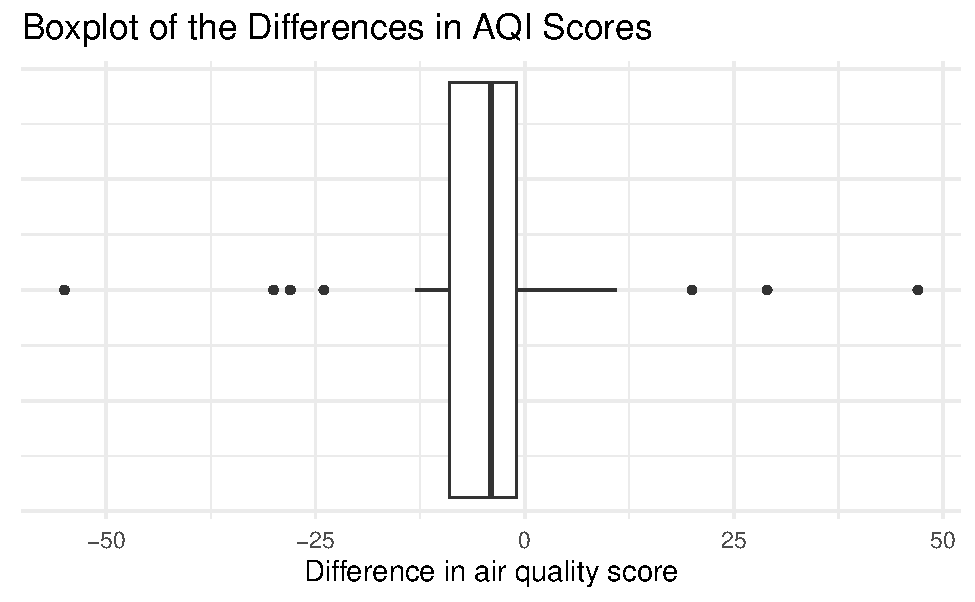
\includegraphics[width=0.7\linewidth]{08-inference-2cat_test_files/figure-latex/unnamed-chunk-2-1} \end{center}

\begin{enumerate}
\def\labelenumi{\arabic{enumi}.}
\setcounter{enumi}{9}
\tightlist
\item
  Fill in the blanks on the graph above with the appropriate variable names and categories to complete the segmented bar plot comparing the proportion of head injuries between those who wear helmets and those who do not wear helmets. \emph{Hint}: Use the conditional proportions from questions 8 and 9.
\end{enumerate}

\vspace{1mm}

\begin{enumerate}
\def\labelenumi{\arabic{enumi}.}
\setcounter{enumi}{10}
\tightlist
\item
  Based on the segmented bar plot, Does there appear to be an association between helmet use and head injury? Explain using the plot.
\end{enumerate}

\vspace{0.7in}

\begin{enumerate}
\def\labelenumi{\arabic{enumi}.}
\setcounter{enumi}{11}
\tightlist
\item
  Calculate the summary statistic for this study. Use helmet use (\texttt{Yes}) minus no helmet use (\texttt{No}) as the order of subtraction.
\end{enumerate}

\vspace{0.4in}

\begin{enumerate}
\def\labelenumi{\arabic{enumi}.}
\setcounter{enumi}{12}
\tightlist
\item
  What is the notation used for the value calculated in question 12?
\end{enumerate}

\vspace{0.1in}

\hypertarget{use-statistical-analysis-methods-to-draw-inferences-from-the-data}{%
\subsubsection*{Use statistical analysis methods to draw inferences from the data}\label{use-statistical-analysis-methods-to-draw-inferences-from-the-data}}
\addcontentsline{toc}{subsubsection}{Use statistical analysis methods to draw inferences from the data}

To test the null hypothesis, we could use simulation-based methods as we did with a single categorical variable in class. In this in-class activity, we will focus on theory-based methods. Like with a single proportion, the sampling distribution of a difference in sample proportions can be mathematically modeled using the normal distribution if certain conditions are met.

Conditions for the sampling distribution of \(\hat{p}_1-\hat{p}_2\) to follow an approximate normal distribution:

\begin{itemize}
\item
  \textbf{Independence}: The data are independent within and between the two groups. (\emph{Remember}: This also must be true to use simulation methods!)
\item
  \textbf{Success-failure condition}: The success-failure condition holds for each group. Under the null hypothesis, the proportions \(\pi_1\) and \(\pi_2\) are equal, so we check the success-failure condition with our best estimate of these values under \(H_0\), the pooled proportion from the two samples,
\end{itemize}

\[
\hat{p}_{pool} = \frac{\text{number of "successes"}}{\text{number of cases}} = \frac{\hat{p}_1 n_1+\hat{p}_2 n_2}{n_1+n_2}
\]
We then check that all four of the following inequalities hold:

\[\hat{p}_{pool} \times n_1 \ge 10, \hspace{1cm} (1 - \hat{p}_{pool}) \times n_1 \geq 10,\]
\[\hat{p}_{pool} \times n_2 \ge 10, \hspace{1cm} (1 - \hat{p}_{pool}) \times n_2 \geq 10\]

\vspace{.1in}

\begin{enumerate}
\def\labelenumi{\arabic{enumi}.}
\setcounter{enumi}{13}
\tightlist
\item
  Is the independence condition met? Explain your answer.
\end{enumerate}

\vspace{0.4in}

\begin{enumerate}
\def\labelenumi{\arabic{enumi}.}
\setcounter{enumi}{14}
\tightlist
\item
  Is the success-failure condition met for each group? Show your work to verify your answer.
\end{enumerate}

\vspace{0.8in}

To calculate the standardized statistic we use:

\[
Z = \frac{\text{point estimate} - \text{null value}}{SE},
\]

where the null standard error is calculated using the pooled proportion of successes:

\[
SE_0(\hat{p}_1-\hat{p}_2)=\sqrt{\hat{p}_{pool}(1-\hat{p}_{pool})\left(\frac{1}{n_1}+\frac{1}{n_2}\right)}.
\]

\newpage

\begin{enumerate}
\def\labelenumi{\arabic{enumi}.}
\setcounter{enumi}{15}
\tightlist
\item
  Calculate \(SE_0(\hat{p}_1-\hat{p}_2)\).
\end{enumerate}

\vspace{1in}

\begin{enumerate}
\def\labelenumi{\arabic{enumi}.}
\setcounter{enumi}{16}
\tightlist
\item
  Calculate the standardized statistic.
\end{enumerate}

\vspace{1in}

We will use the \texttt{pnorm} function in \texttt{R} to find the p-value. Use the provided \texttt{R} script file and enter the value of the standardized statistic found in question 17 at \texttt{xx} in line 27; highlight and run lines 27--29.

\begin{Shaded}
\begin{Highlighting}[]
\KeywordTok{pnorm}\NormalTok{(xx, }\CommentTok{\# Enter value of standardized statistic}
      \DataTypeTok{m=}\DecValTok{0}\NormalTok{, }\DataTypeTok{s=}\DecValTok{1} \CommentTok{\# Using the standard normal mean = 0, sd = 1}
      \DataTypeTok{lower.tail=}\OtherTok{TRUE}\NormalTok{) }\CommentTok{\# Gives a p{-}value less than the standardized statistic}
\end{Highlighting}
\end{Shaded}

\begin{enumerate}
\def\labelenumi{\arabic{enumi}.}
\setcounter{enumi}{17}
\item
  Report the p-value from the \texttt{R} output.
  \vspace{0.2in}
\item
  Interpret the p-value in context of the study.
\end{enumerate}

\vspace{1in}

\begin{enumerate}
\def\labelenumi{\arabic{enumi}.}
\setcounter{enumi}{19}
\tightlist
\item
  How much evidence does the p-value provide against the null hypothesis? \emph{Hint}: Refer to the guidelines given in Activity 6.
\end{enumerate}

\vspace{0.4in}

\begin{enumerate}
\def\labelenumi{\arabic{enumi}.}
\setcounter{enumi}{20}
\tightlist
\item
  Write a conclusion to the test.
\end{enumerate}

\vspace{1in}

\newpage

\hypertarget{types-of-errors}{%
\subsubsection*{Types of errors}\label{types-of-errors}}
\addcontentsline{toc}{subsubsection}{Types of errors}

Hypothesis tests are not flawless. In a hypothesis test, there are two competing hypotheses: the null and alternative. We make a decision about which might be true, but we may choose incorrectly.

\begin{table}
\caption{Four different possible scenarios for hypothesis test decisions.}
\centering
\begin{tabular}[h]{ll|cc}
\hline
 & &  \multicolumn{2}{c}{\textbf{Test conclusion}} \\
 &  & \multicolumn{1}{c}{Fail to reject $H_0$} & \multicolumn{1}{c}{Reject $H_0$}\\
\hline
 & $H_0$ true & Good decision & Type 1 Error\\
\hline
\textbf{Truth} & $H_A$ true & Type 2 Error & Good decision\\
\hline
\end{tabular}
\label{tab:errors}
\end{table}

Shown in Table \ref{tab:errors}, a \textbf{Type 1 Error} happens when we reject the null hypothesis when \(H_0\) is actually true. A \textbf{Type 2 Error} happens when we fail to reject the null hypothesis when the alternative is actually true.

\begin{enumerate}
\def\labelenumi{\arabic{enumi}.}
\setcounter{enumi}{21}
\tightlist
\item
  Using a significance level of 0.05, based on the p-value found in question 18, what decision do you make in regards to the null hypothesis?
\end{enumerate}

\vspace{0.3in}

\begin{enumerate}
\def\labelenumi{\arabic{enumi}.}
\setcounter{enumi}{22}
\tightlist
\item
  What type of error could we have made?
\end{enumerate}

\vspace{0.3in}

\begin{enumerate}
\def\labelenumi{\arabic{enumi}.}
\setcounter{enumi}{23}
\tightlist
\item
  Write this error in context of the problem.
\end{enumerate}

\vspace{0.8in}

\begin{enumerate}
\def\labelenumi{\arabic{enumi}.}
\setcounter{enumi}{24}
\tightlist
\item
  Write a paragraph summarizing the results of the study as if writing a press release. Be sure to describe:
\end{enumerate}

\begin{itemize}
\item
  Summary statistic
\item
  Test statistic and interpretation
\item
  P-value and interpretation
\item
  Conclusion (written to answer the research question)
\item
  Scope of inference
\end{itemize}

\vspace{2in}

\newpage

\hypertarget{out-of-class-activity}{%
\subsection{Out-of-class activity}\label{out-of-class-activity}}

The remaining questions cover simulation-based methods for testing two categorical variables. Use Section 5.4.3 in the textbook and the TwoPropSim video to complete the following questions.

\begin{enumerate}
\def\labelenumi{\arabic{enumi}.}
\item
  First let's think about how one simulation would be created on the null distribution using cards.

  How many cards would you need?
  \vspace{0.1in}

  What would be written on each card?
\end{enumerate}

\vspace{0.5in}

\begin{enumerate}
\def\labelenumi{\arabic{enumi}.}
\setcounter{enumi}{1}
\tightlist
\item
  Next, we would mix the cards together and shuffle into two piles. How many cards would be in each pile? What would each pile represent?
\end{enumerate}

\vspace{0.8in}

\begin{enumerate}
\def\labelenumi{\arabic{enumi}.}
\setcounter{enumi}{2}
\tightlist
\item
  Once we have one simulated sample, what would we calculate and plot on the null distribution? \emph{Hint}: What statistic are we calculating from the data?
\end{enumerate}

\vspace{0.8in}

To create the null distribution of sample differences in proportions, we will use the \texttt{two\_proportion\_test} function in \texttt{R} (in the \texttt{catstats} package). We will need to enter the response variable name and the explanatory variable name for the formula, the data set name identified above as \texttt{injury}, the outcome for the explanatory variable to give the order of subtraction for First in Subtraction, number of repetitions, the outcome for the response variable that is a success for Response Value Numerator, and the direction of the alternative hypothesis.

The response variable name is Outcome and the explanatory variable name is Helmet.

\newpage

\begin{enumerate}
\def\labelenumi{\arabic{enumi}.}
\setcounter{enumi}{3}
\tightlist
\item
  What inputs should be entered for each of the following to create the simulation?
\end{enumerate}

\vspace{.2in}

\begin{itemize}
\tightlist
\item
  First in Subtraction (What is the outcome for the explanatory variable that is used as first in the order of subtraction? \texttt{"Yes"} or \texttt{"No"}):
\end{itemize}

\vspace{.2in}

\begin{itemize}
\tightlist
\item
  Number of repetitions:
\end{itemize}

\vspace{.2in}

\begin{itemize}
\tightlist
\item
  Response Value Numerator (What is the outcome for the response variable that is considered a success? \texttt{"Head\ Injury"} or \texttt{"No\ Head\ Injury"}):
\end{itemize}

\vspace{.2in}

\begin{itemize}
\tightlist
\item
  As extreme as (enter the value for the sample difference in proportions):
\end{itemize}

\vspace{.2in}

\begin{itemize}
\tightlist
\item
  Direction (\texttt{"greater"}, \texttt{"less"}, or \texttt{"two-sided"}):
\end{itemize}

\vspace{.2in}

Using the \texttt{R} script file for this activity, enter your answers for question 4 in place of the xx's in the two proportion test code to produce the null distribution with 1000 simulations, highlight and run lines 1--12 and then 33--39.

\begin{Shaded}
\begin{Highlighting}[]
\KeywordTok{two\_proportion\_test}\NormalTok{(}\DataTypeTok{formula =}\NormalTok{ Outcome }\OperatorTok{\textasciitilde{}}\StringTok{ }\NormalTok{Helmet, }\CommentTok{\# response\textasciitilde{}explanatory}
                    \DataTypeTok{data=}\NormalTok{ injury, }\CommentTok{\# Name of dataset}
                    \DataTypeTok{first\_in\_subtraction =} \StringTok{"xx"}\NormalTok{, }\CommentTok{\# Order of subtraction: enter the name of Group 1}
                    \DataTypeTok{number\_repetitions =} \DecValTok{1000}\NormalTok{, }\CommentTok{\# Always use a minimum of 1000 repetitions}
                    \DataTypeTok{response\_value\_numerator =} \StringTok{"xx"}\NormalTok{, }\CommentTok{\# Define which outcome is a success }
                    \DataTypeTok{as\_extreme\_as =}\NormalTok{ xx, }\CommentTok{\# Type your calculated observed statistic (difference in sample proportions)}
                    \DataTypeTok{direction=}\StringTok{"xx"}\NormalTok{) }\CommentTok{\# Alternative hypothesis direction ("greater","less","two{-}sided")}
\end{Highlighting}
\end{Shaded}

\begin{enumerate}
\def\labelenumi{\arabic{enumi}.}
\setcounter{enumi}{4}
\tightlist
\item
  Sketch the null distribution created here.
\end{enumerate}

\newpage

\begin{enumerate}
\def\labelenumi{\arabic{enumi}.}
\setcounter{enumi}{5}
\tightlist
\item
  What value is the null distribution centered around? Explain why this makes sense?
\end{enumerate}

\vspace{1in}

\begin{enumerate}
\def\labelenumi{\arabic{enumi}.}
\setcounter{enumi}{6}
\tightlist
\item
  What is the p-value? \emph{Remember}: This is the value given at the bottom of the null distribution.
\end{enumerate}

\vspace{0.2in}

\begin{enumerate}
\def\labelenumi{\arabic{enumi}.}
\setcounter{enumi}{7}
\tightlist
\item
  Is the p-value found in question 7 for the out-of-class activity similar to the p-value found using the theory-based test? Explain why you would expect this to be true.
\end{enumerate}

\vspace{1in}

\hypertarget{take-home-messages}{%
\subsection{Take-home messages}\label{take-home-messages}}

\begin{enumerate}
\def\labelenumi{\arabic{enumi}.}
\item
  When comparing two groups, we are looking at the relationship between two parameters. In the null hypothesis we assume the two parameters are equal or that there is no difference between the two proportions.
\item
  We use the same guidelines for the strength of evidence as we did in activity 6.
\item
  The standardized statistic when the response variable is categorical is a Z score and compared to the standard normal distribution to find the p-value. To find the standardardized statistic we take the value of the statistic minus the null value, divided by the standard error of the statistic. The standardized statistic measures the number of standard errors the statistic is from the null value.
\item
  If we make the decision to reject the null hypothesis (the p-value is less than the significance level), we could have a possible Type 1 error.
\item
  If we make the decision to fail to reject the null hypothesis (the p-value is greater than the significance leve), we could have a possible Type 2 error.
\end{enumerate}

\hypertarget{additional-notes}{%
\subsection{Additional notes}\label{additional-notes}}

Use this space to summarize your thoughts and take additional notes on this week's activity and material covered.

\end{document}
